\documentclass{dense_template}
\newcommand*{\name}{Felipe Alejandro Jiménez Castillo}
\newcommand*{\code}{215671386}
\newcommand*{\school}{Universidad de Guadalajara - CUCEI}
\newcommand*{\course}{Computación Tolerante a Fallas}
\newcommand*{\assignment}{Herramientas para el Manejo de Errores}
\renewcommand{\contentsname}{Contenido}

\begin{document}
\maketitle
%%%%%%%%%%%%%%%%%%%%
\tableofcontents
\newpage
%%%%%%%%%%%%%%%%%%%%
\section{Introducción}
El manejo de errores hace referencia a la respuesta y recuperación presentes en las condiciones de error que se encuentra un programa o software, en otras palabras es el proceso compuesto por la anticipación, detección y resolución de diferentes tipos de errores en una aplicación y/o programa. El manejo de errores nos ayuda a mantener el flujo de ejecución adecuado de un programa. En el día a día, muchas aplicaciones enfrentan numerosos retos de diseño cuando se consideran técnicas de manejo de errores, es por esto, que es todo una ciencia y arte conocer dichas técnicas para una implementación concisa.  
%%%%%%%%%%%%%%%%%%%%
\section{Desarrollo}
Los lenguajes de programación modernos, y no tan modernos, están diseñados o se van mejorando, respecto a sus versiones previas, con muchas utilidades que, seguramente, automatizan procesos, los hacen más seguros o incluso suplen procesos. Es aquí donde muchas de las mejoras también son para el tratamiento de errores; Nuevos manejos de errores, nuevas formas de tener más retroalimentación y demás. De manera concisa mencionaré 2 de las inclusiones en algunos lenguajes que me parecen interesantes y no tan comunes.
\begin{enumerate}
    \item \textbf{Error}
    \begin{enumerate}
        \item La función \textit{Error}, en lenguajes de Programación Funcional, funciona como una sentencia de escape que genera un error con mensajes personalizados, de forma que podamos interrumpir la ejecución de un programa con la resolución y retroalimentación buscada. Similar a \textit{Error}, está \textit{throw} en los lenguajes de programación no funcional, pero este no necesita de instrucciones que atrapen el error, si no que causa la evaluación de un paro y cracheo.
    \end{enumerate}
    \begin{center}
        \vspace{0.5cm}
        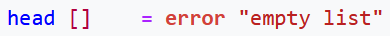
\includegraphics[width=0.4\textwidth]{error.png}
    \end{center}
    \item \textbf{Maybe}
    \begin{enumerate}
        \item Este tipo de dato, comúnmente visto en los lenguajes de \textit{Programación Funcional}, representa que cierto dato puede ser \textit{Nothing (NULL)} o un \textit{Just a (Just es un constructor de un tipo de dato anónimo, el cual será inicializado con el valor de 'a')}, lo que nos permite una conjunción de más casos de uso, sin necesidad de errores o excepciones. En lenguajes de programación no funcional, el tipo de dato \textit{Maybe} puede ser visto como una unión o como un acceso a poder retornar \textit{NULL} para especificar que un valor puede, o no, estar ahí. Finalmente podemos definir un dato como \textit{\textbf{data Maybe a = Just a $\mid$  Nothing}}, haciendo elusión a que puede ser cierto tipo de dato o nada.
    \end{enumerate}
        \begin{center}
        \vspace{0.5cm}
        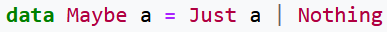
\includegraphics[width=0.4\textwidth]{Maybe.png}
    \end{center}
\end{enumerate}
%%%%%%%%%%%%%%%%%%%%
\pagebreak
%%%%%%%%%%%%%%%%%%%%
\section{Conclusión}
\textit{Maybe} y \textit{Error} son dos características importantes de \textit{Haskell} que ayudan a los programadores a escribir código más robusto y fiable. Así mismo estás herramientas de código hacen el código más seguro, ya que obligan a los programadores a manejar errores explícitamente, de manera que se previenen daños, además de constar de una característica muy deseable, la modularidad, ya que con esto también se provee al programador con una forma de encapsular errores dentro de tipos de datos específicos, haciendo el código más expresivo y descriptivo.
%%%%%%%%%%%%%%%%%%%%
\pagebreak
%%%%%%%%%%%%%%%%%%%%
\section{Bilbiografia}
\sloppy
\begin{enumerate}
    \item Handling errors in Haskell. (n.d.). Haskell.org. Retrieved August 28, 2023, from https://wiki.haskell.org/Handling\_errors\_in\_Haskell
    \item Maybe. (n.d.). Haskell.org. Retrieved August 28, 2023, from https://wiki.haskell.org/Maybe
    \item Villa, J. P. (n.d.). Errors and exceptions in Haskell. Stackbuilders.com. Retrieved August 28, 2023, from https://www.stackbuilders.com/blog/errors-and-exceptions-in-haskell/
\end{enumerate}
\end{document}

